\documentclass[11pt,letterpaper]{article}

% include figures
\usepackage{graphicx}
% get nice colors
\usepackage{xcolor}

% change default font to Palatino (looks nicer!)
\usepackage[latin1]{inputenc}
\usepackage{mathpazo}
\usepackage[T1]{fontenc}
% load some useful math symbols/fonts
\usepackage{latexsym,amsfonts,amsmath,amssymb,wasysym}
% be able to insert code
\usepackage{listings}

% comfort package to easily set margins
\usepackage[top=1in, bottom=1in, left=1in, right=1in]{geometry}

% spacing after a paragraph
\setlength{\parskip}{.15cm}
% indentation at the top of a new paragraph
\setlength{\parindent}{0.0cm}
% make units not slanted in math mode
\newcommand{\unit}[1]{\ensuremath{\, \mathrm{#1}}}

\begin{document}

\begin{center}
\Large
Ay190 -- Worksheet 14\\
Daniel DeFelippis\\
Date: \today
\end{center}

%%
%%
%% I worked with Scott Barenfeld
%%
%% All python code can be found in the ws14 directory in my repository
%%
%%

\section*{Advection Equation 2: Electric Burger-loo}

We are solving Burger's equation:
$$ \frac{\partial u}{\partial t} + u\frac{\partial u}{\partial x} = 0, $$
with the initial condition 
$$ \Psi(x,t=0) = \frac{1}{8} \sin\left(\frac{2\pi x}{L}\right), $$
where $L=100$ on the domain $[0,L]$. Like worksheet 11, we use outflow 
boundary conditions, represented by the function "apply\_bcs(y)" defined by the code:
\lstinputlisting[language=Python, firstline=10, lastline=11]{ws14.py}
which uses the value of the function in the last interior grid points 
as the value at the boundary points.

There are two changes from this code and the code for worksheet 11. First, "dt" is 
defined using the maximum value of $\Psi(x,t=0)$ because we want a constant dt for all
grid points. This done with the line:
\lstinputlisting[language=Python, firstline=31, lastline=31]{ws14.py}.
The other change is in calculating the upwind gridpoints. The velocity is not always the
same sign in this case, which means that the direction opposite of the velocity will 
change here as opposed to worksheet 11. Therefore, we need to check the sign of 
the velocity and adjust how we calculate the upwind gridpoints appropriately:
\lstinputlisting[language=Python, firstline=56, lastline=62]{ws14.py}.

Running the code, we see that the two sides of the $\sin$ function, after starting out 
evenly (figure~\ref{fig:t=0}) start to push towards each other 
(figures~\ref{fig:t=40} and \ref{fig:t=80}). At $t = 120$ we see that the 
center of the time-evolved function looks almost vertical (figure~\ref{fig:t=120}). 
At about $t=140$, a jump (the shock) appears, evidenced by the fact that the center of 
the function is devoid of any crosses indicating data points: they've all 
migrated to one side of the jump (figure~\ref{fig:t=140}). 
By $t=160$ it is solidly there (figure~\ref{fig:t=160}).
So, using the upwind scheme, we've demonstrated that around $t=140$ a shock forms in the 
solution to Burger's equation for this $\sin$ wave.

\begin{figure}[bth]
\centering
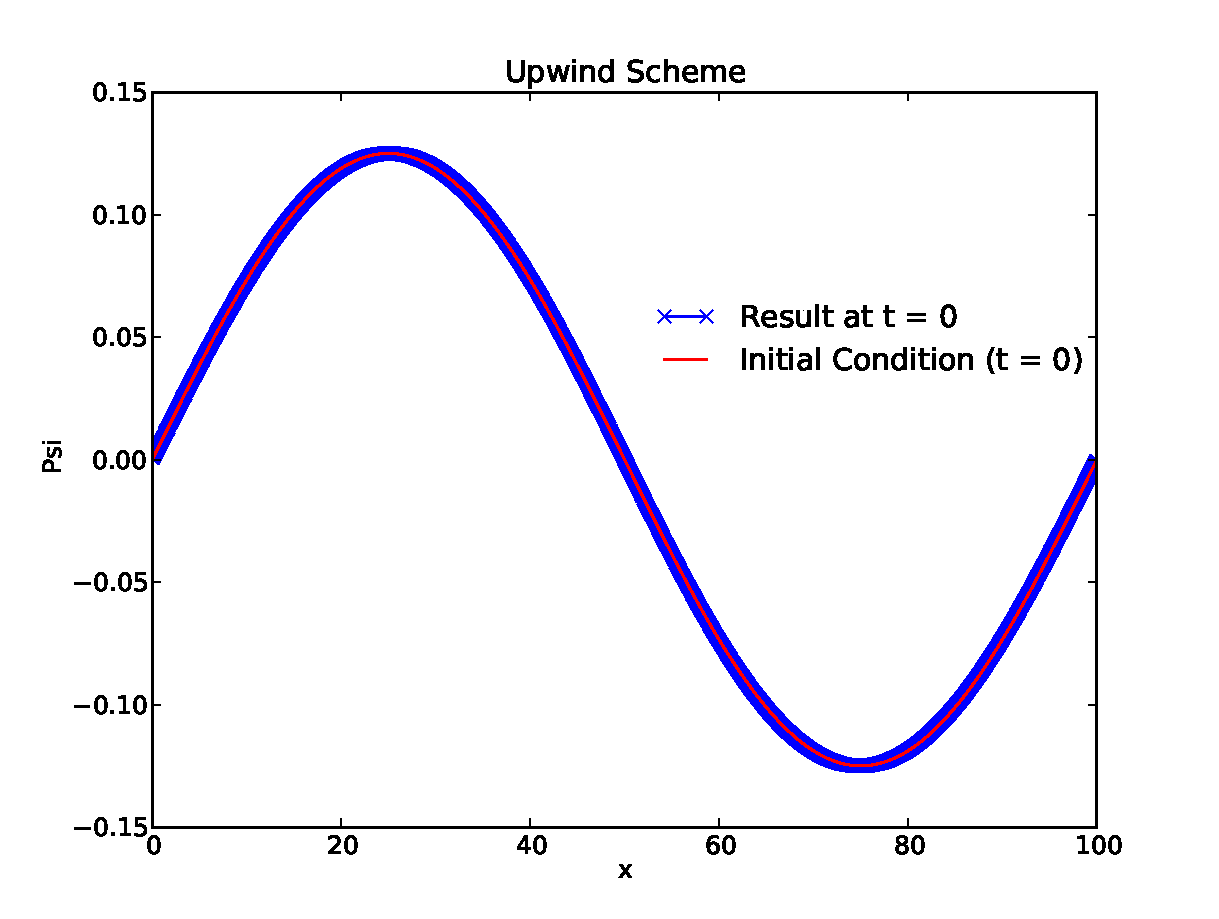
\includegraphics[width=0.80\textwidth]{t=0.pdf}
\caption{Plot of $\Psi$ at $t = 0$.}
\label{fig:t=0}
\end{figure}

\begin{figure}[bth]
\centering
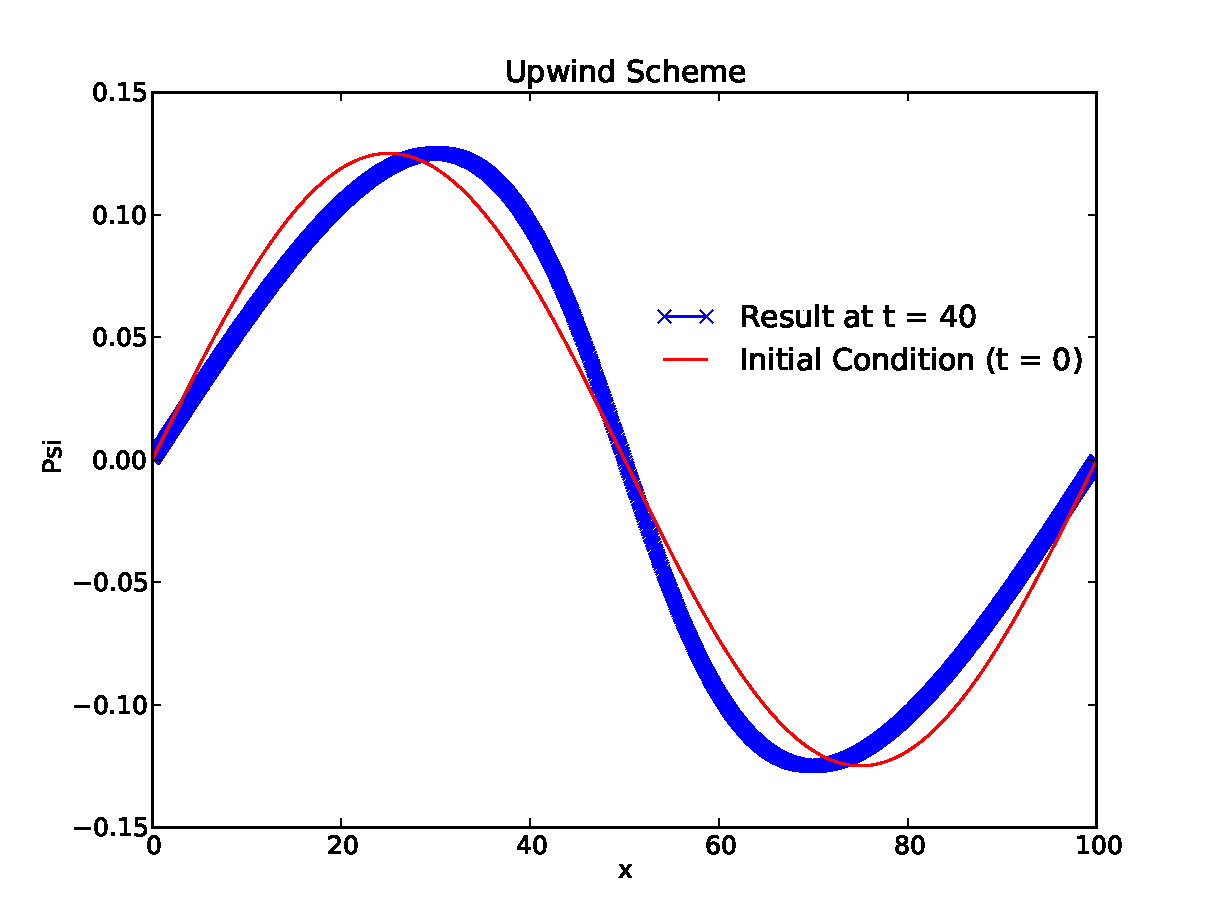
\includegraphics[width=0.80\textwidth]{t=40.pdf}
\caption{Plot of $\Psi$ at $t = 40$ and initial condition.}
\label{fig:t=40}
\end{figure}

\begin{figure}[bth]
\centering
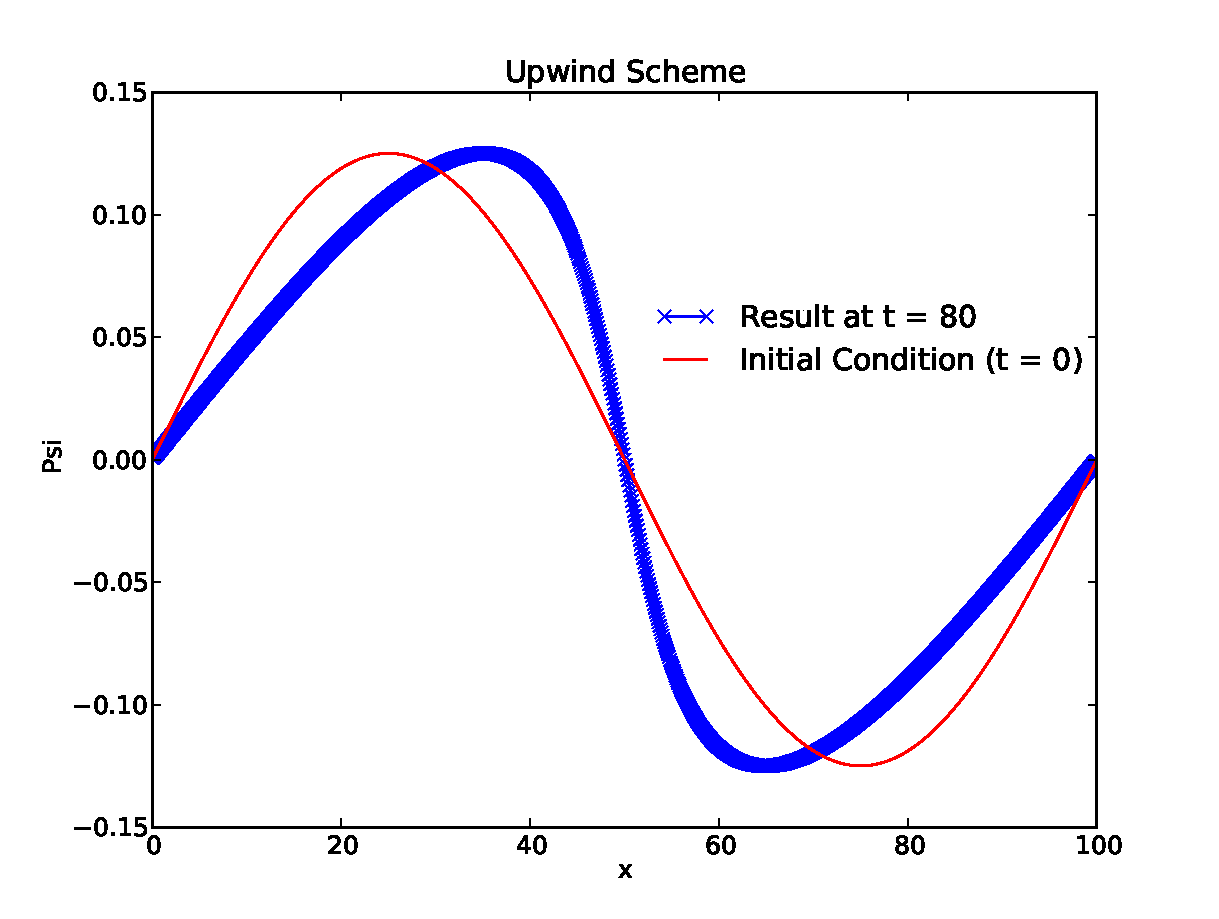
\includegraphics[width=0.80\textwidth]{t=80.pdf}
\caption{Plot of $\Psi$ at $t = 80$ and initial condition.}
\label{fig:t=80}
\end{figure}

\begin{figure}[bth]
\centering
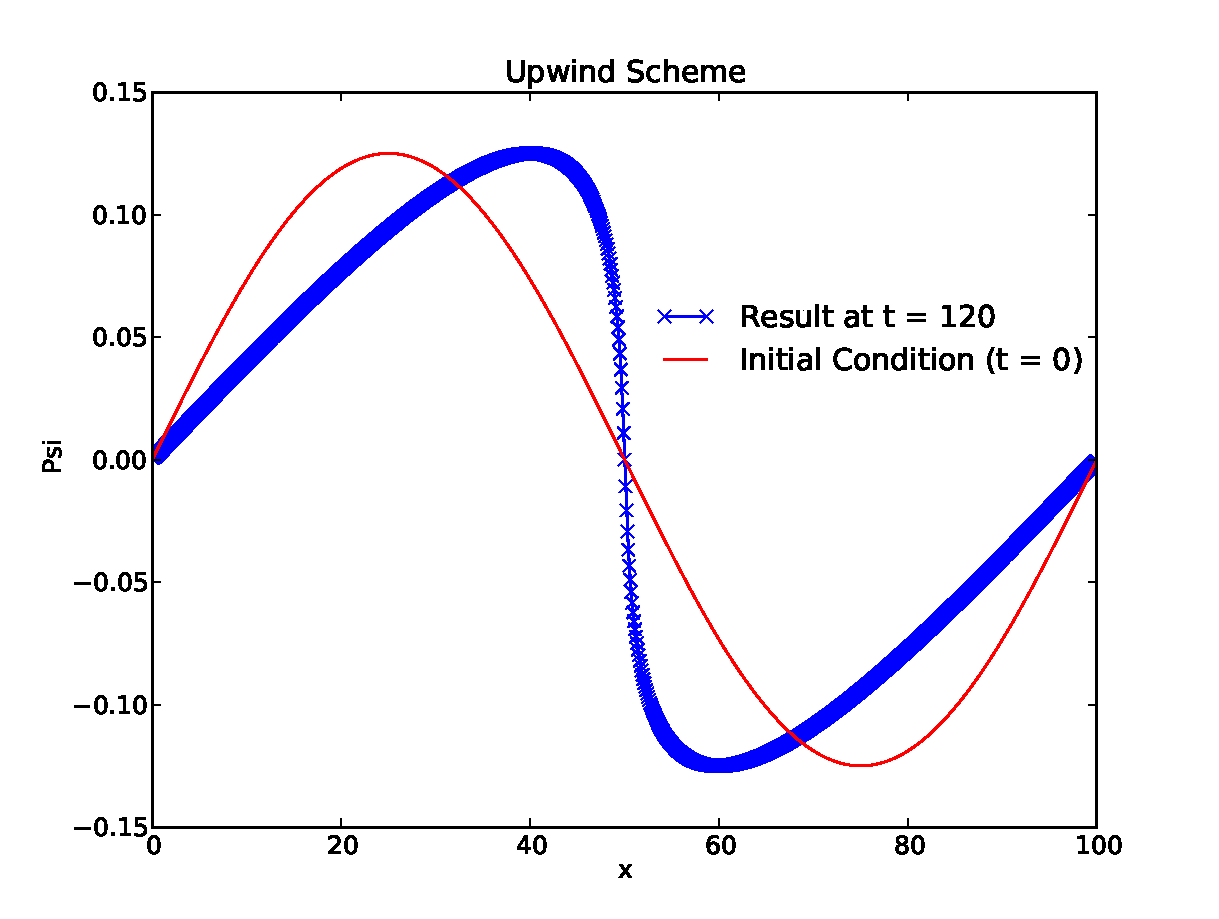
\includegraphics[width=0.80\textwidth]{t=120.pdf}
\caption{Plot of $\Psi$ at $t = 120$ and initial condition.}
\label{fig:t=120}
\end{figure}

\begin{figure}[bth]
\centering
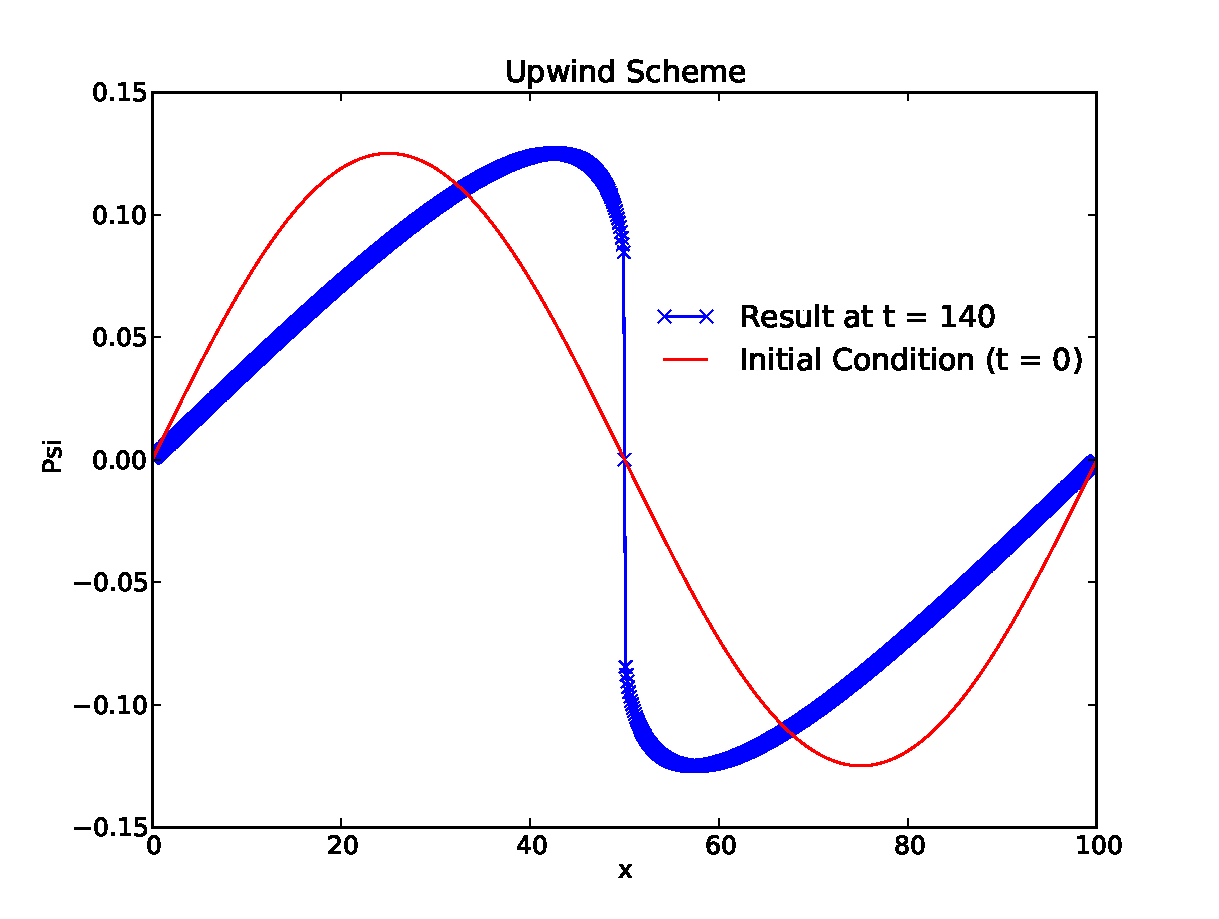
\includegraphics[width=0.80\textwidth]{t=140.pdf}
\caption{Plot of $\Psi$ at $t = 140$ and initial condition.}
\label{fig:t=140}
\end{figure}

\begin{figure}[bth]
\centering
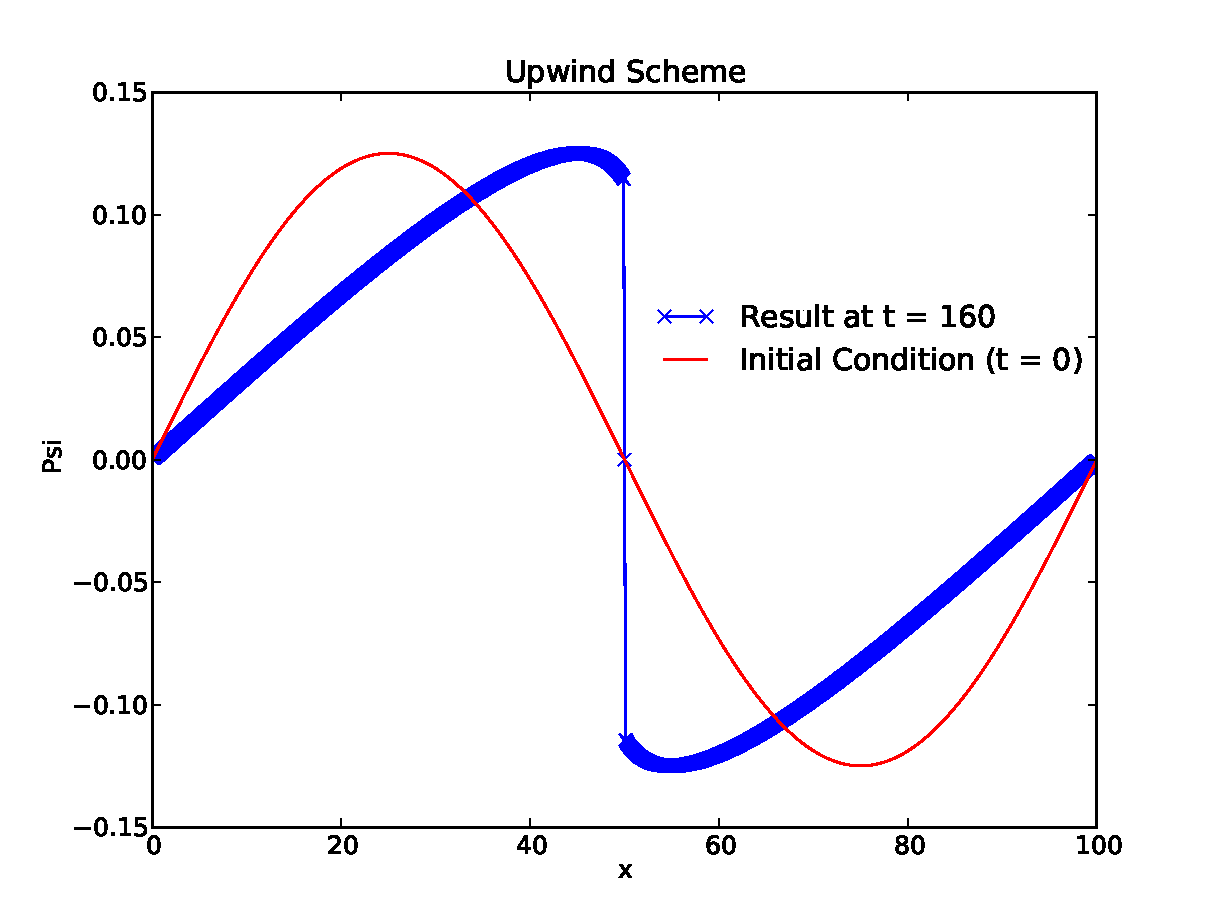
\includegraphics[width=0.80\textwidth]{t=160.pdf}
\caption{Plot of $\Psi$ at $t = 160$ and initial condition.}
\label{fig:t=160}
\end{figure}

\end{document}
